\documentclass{standalone}
\usepackage{tikz}
\usetikzlibrary{patterns, positioning}
\usepackage[sfdefault]{ClearSans} %% option 'sfdefault' activates Clear Sans as the default text font
\usepackage[T1]{fontenc}

\begin{document}
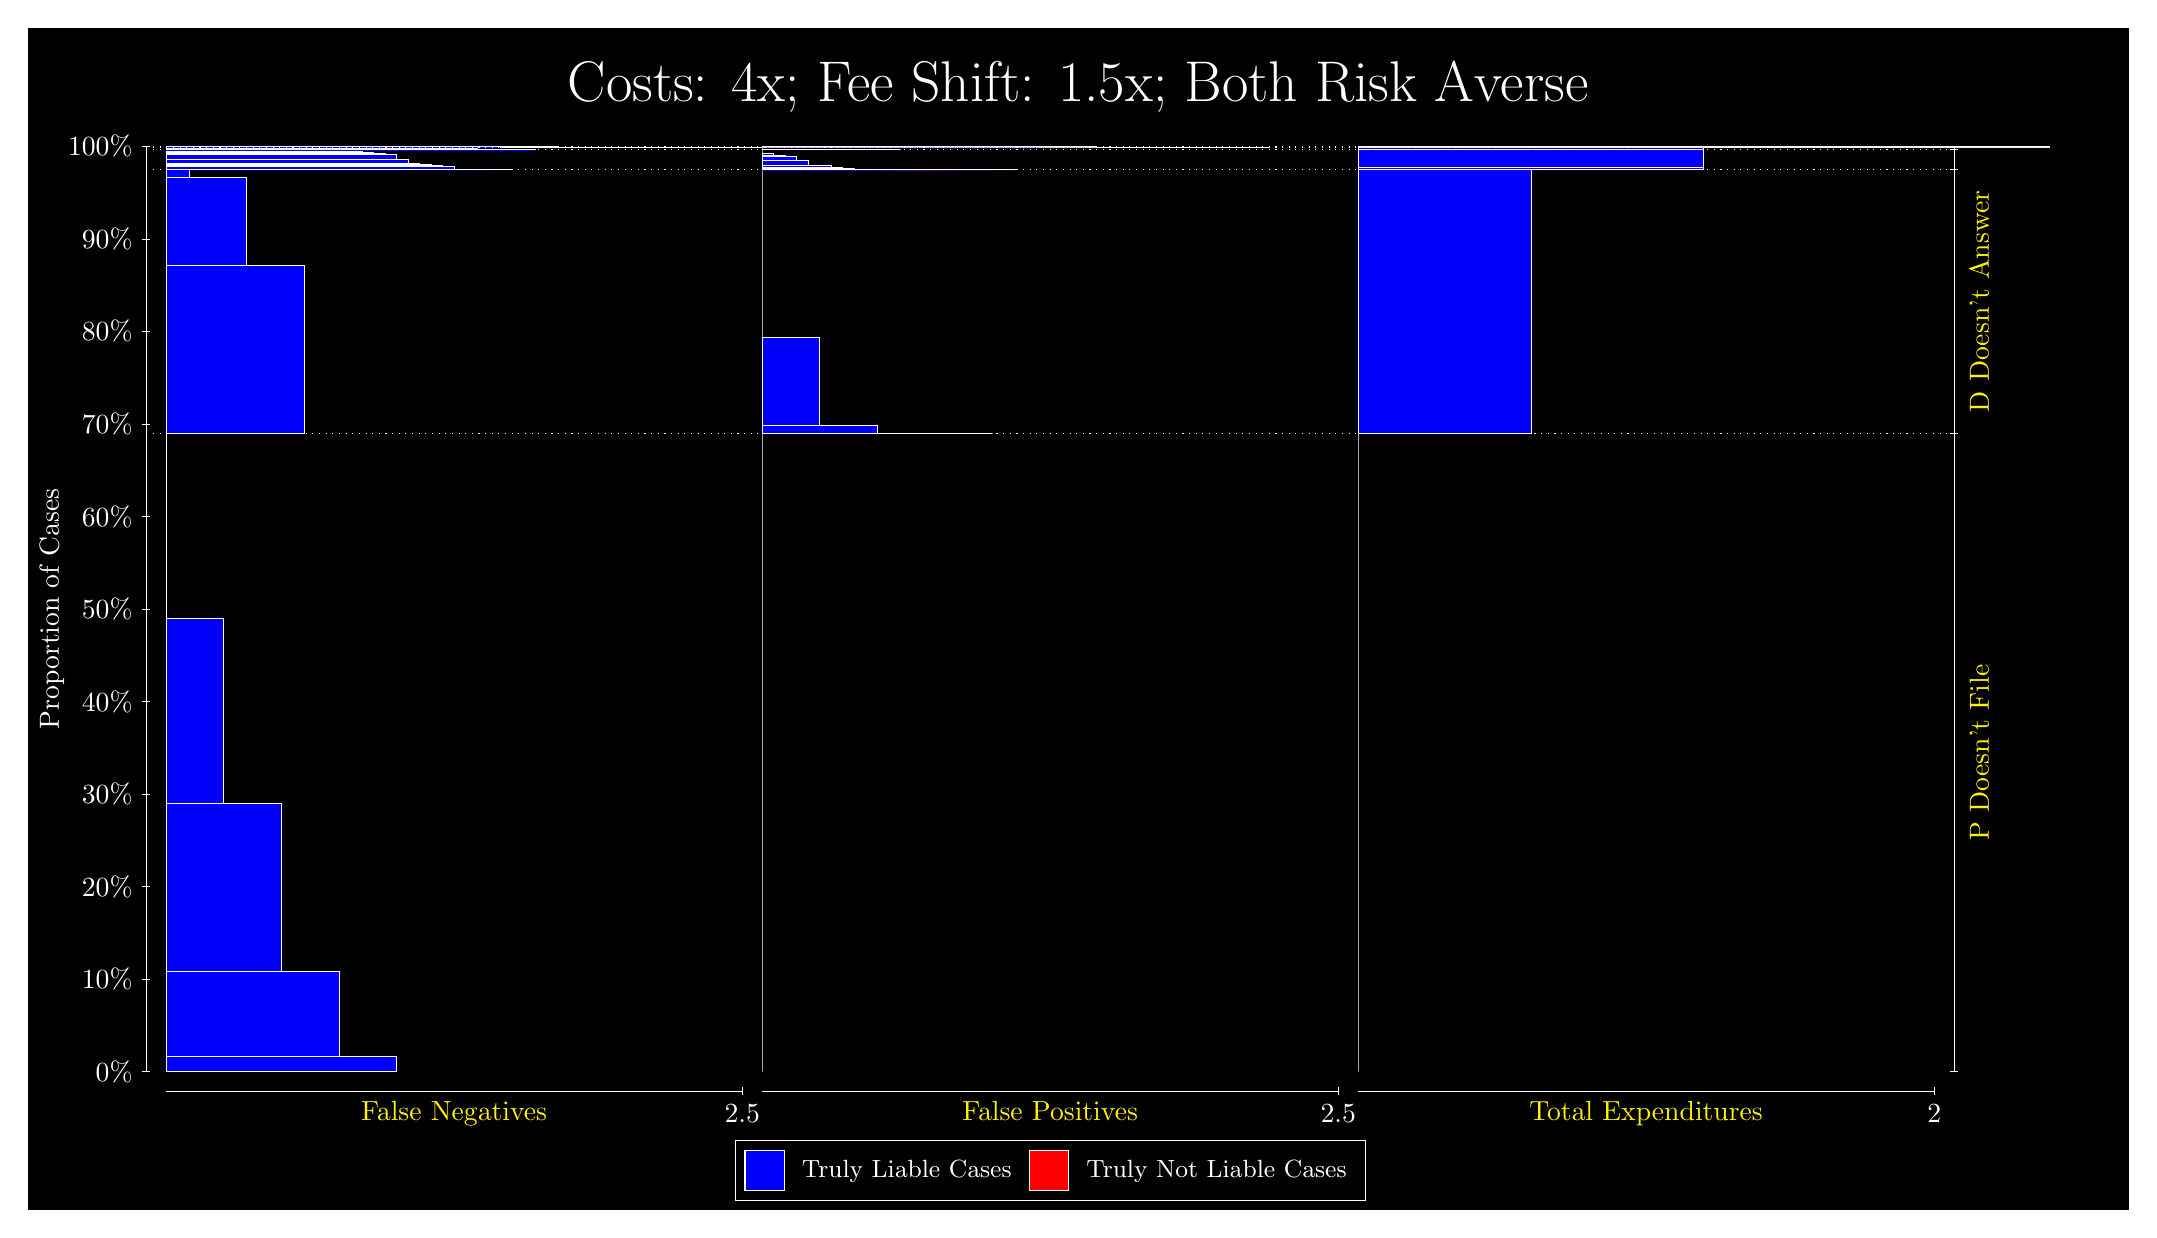
\begin{tikzpicture}
\draw[fill=black] (0,0) rectangle (26.667,15);
\draw[text=white] (0,13.5) rectangle (26.667,15) node[midway] {\huge Costs: 4x; Fee Shift: 1.5x; Both Risk Averse};
\draw[white, very thin] (1.5,1.75) -- (1.5,13.5);
\node[rotate=90, text=white, anchor=center] at (0.3, 7.625) {Proportion of Cases};
\draw[white, very thin] (1.45,1.75) -- (1.55,1.75);
\node[text=white, anchor=east] at (1.45, 1.75) {0\%};
\draw[white, very thin] (1.45,2.925) -- (1.55,2.925);
\node[text=white, anchor=east] at (1.45, 2.925) {10\%};
\draw[white, very thin] (1.45,4.1) -- (1.55,4.1);
\node[text=white, anchor=east] at (1.45, 4.1) {20\%};
\draw[white, very thin] (1.45,5.275) -- (1.55,5.275);
\node[text=white, anchor=east] at (1.45, 5.275) {30\%};
\draw[white, very thin] (1.45,6.45) -- (1.55,6.45);
\node[text=white, anchor=east] at (1.45, 6.45) {40\%};
\draw[white, very thin] (1.45,7.625) -- (1.55,7.625);
\node[text=white, anchor=east] at (1.45, 7.625) {50\%};
\draw[white, very thin] (1.45,8.8) -- (1.55,8.8);
\node[text=white, anchor=east] at (1.45, 8.8) {60\%};
\draw[white, very thin] (1.45,9.975) -- (1.55,9.975);
\node[text=white, anchor=east] at (1.45, 9.975) {70\%};
\draw[white, very thin] (1.45,11.15) -- (1.55,11.15);
\node[text=white, anchor=east] at (1.45, 11.15) {80\%};
\draw[white, very thin] (1.45,12.325) -- (1.55,12.325);
\node[text=white, anchor=east] at (1.45, 12.325) {90\%};
\draw[white, very thin] (1.45,13.5) -- (1.55,13.5);
\node[text=white, anchor=east] at (1.45, 13.5) {100\%};

\draw[white, very thin] (24.457,1.75) -- (24.457,13.5);
\draw[white, very thin] (24.407,1.75) -- (24.507,1.75);
\node[anchor=west] at (24.407, 1.75) {};
\draw[white, very thin] (24.407,9.8584) -- (24.507,9.8584);
\node[anchor=west] at (24.407, 9.8584) {};
\draw[white, very thin] (24.407,13.205) -- (24.507,13.205);
\node[anchor=west] at (24.407, 13.205) {};
\draw[white, very thin] (24.407,13.458) -- (24.507,13.458);
\node[anchor=west] at (24.407, 13.458) {};
\draw[white, very thin] (24.407,13.487) -- (24.507,13.487);
\node[anchor=west] at (24.407, 13.487) {};
\draw[white, very thin] (24.407,13.494) -- (24.507,13.494);
\node[anchor=west] at (24.407, 13.494) {};
\draw[white, very thin] (24.407,13.5) -- (24.507,13.5);
\node[anchor=west] at (24.407, 13.5) {};

\draw[white, very thin, fill=blue] (1.75,1.75) rectangle (4.6775,1.9458);
\draw[white, very thin, fill=blue] (1.75,1.9458) rectangle (3.9457,3.0214);
\draw[white, very thin, fill=blue] (1.75,3.0214) rectangle (3.2138,5.1601);
\draw[white, very thin, fill=blue] (1.75,5.1601) rectangle (2.4819,7.5084);
\draw[white, very thin, fill=red] (1.75,7.5084) rectangle (1.75,7.5084);
\draw[white, very thin, fill=blue] (1.75,7.5084) rectangle (1.75,9.8584);
\draw[white, very thin, fill=blue] (1.75,9.8584) rectangle (3.5065,11.986);
\draw[white, very thin, fill=blue] (1.75,11.986) rectangle (2.7746,13.103);
\draw[white, very thin, fill=blue] (1.75,13.103) rectangle (2.0428,13.205);
\draw[white, very thin, fill=red] (1.75,13.205) rectangle (1.75,13.205);
\draw[white, very thin, fill=blue] (1.75,13.205) rectangle (1.75,13.205);
\draw[white, very thin, fill=blue] (1.75,13.205) rectangle (6.1413,13.205);
\draw[white, very thin, fill=blue] (1.75,13.205) rectangle (5.8486,13.205);
\draw[white, very thin, fill=blue] (1.75,13.205) rectangle (5.5558,13.208);
\draw[white, very thin, fill=blue] (1.75,13.208) rectangle (5.4094,13.248);
\draw[white, very thin, fill=blue] (1.75,13.248) rectangle (5.2631,13.257);
\draw[white, very thin, fill=blue] (1.75,13.257) rectangle (5.1167,13.275);
\draw[white, very thin, fill=blue] (1.75,13.275) rectangle (4.9703,13.287);
\draw[white, very thin, fill=blue] (1.75,13.287) rectangle (4.8239,13.334);
\draw[white, very thin, fill=blue] (1.75,13.334) rectangle (4.6775,13.401);
\draw[white, very thin, fill=blue] (1.75,13.401) rectangle (4.5312,13.407);
\draw[white, very thin, fill=blue] (1.75,13.407) rectangle (4.3848,13.425);
\draw[white, very thin, fill=blue] (1.75,13.425) rectangle (4.2384,13.438);
\draw[white, very thin, fill=blue] (1.75,13.438) rectangle (4.092,13.456);
\draw[white, very thin, fill=blue] (1.75,13.456) rectangle (3.9457,13.457);
\draw[white, very thin, fill=blue] (1.75,13.457) rectangle (3.7993,13.457);
\draw[white, very thin, fill=blue] (1.75,13.457) rectangle (3.6529,13.457);
\draw[white, very thin, fill=blue] (1.75,13.457) rectangle (3.5065,13.458);
\draw[white, very thin, fill=blue] (1.75,13.458) rectangle (3.3602,13.458);
\draw[white, very thin, fill=blue] (1.75,13.458) rectangle (3.2138,13.458);
\draw[white, very thin, fill=blue] (1.75,13.458) rectangle (3.0674,13.458);
\draw[white, very thin, fill=blue] (1.75,13.458) rectangle (2.921,13.458);
\draw[white, very thin, fill=blue] (1.75,13.458) rectangle (2.7746,13.458);
\draw[white, very thin, fill=blue] (1.75,13.458) rectangle (2.6283,13.458);
\draw[white, very thin, fill=blue] (1.75,13.458) rectangle (2.3355,13.458);
\draw[white, very thin, fill=blue] (1.75,13.458) rectangle (2.0428,13.458);
\draw[white, very thin, fill=red] (1.75,13.458) rectangle (1.75,13.458);
\draw[white, very thin, fill=blue] (1.75,13.458) rectangle (6.4341,13.459);
\draw[white, very thin, fill=blue] (1.75,13.459) rectangle (5.7022,13.479);
\draw[white, very thin, fill=blue] (1.75,13.479) rectangle (4.9703,13.486);
\draw[white, very thin, fill=blue] (1.75,13.486) rectangle (4.2384,13.487);
\draw[white, very thin, fill=blue] (1.75,13.487) rectangle (3.5065,13.487);
\draw[white, very thin, fill=red] (1.75,13.487) rectangle (1.75,13.487);
\draw[white, very thin, fill=blue] (1.75,13.487) rectangle (3.5065,13.487);
\draw[white, very thin, fill=blue] (1.75,13.487) rectangle (2.7746,13.494);
\draw[white, very thin, fill=blue] (1.75,13.494) rectangle (2.0428,13.494);
\draw[white, very thin, fill=red] (1.75,13.494) rectangle (1.75,13.494);
\draw[white, very thin, fill=blue] (1.75,13.494) rectangle (1.75,13.494);
\draw[white, very thin, fill=blue] (1.75,13.494) rectangle (13.46,13.494);
\draw[white, very thin, fill=blue] (1.75,13.494) rectangle (12.728,13.494);
\draw[white, very thin, fill=blue] (1.75,13.494) rectangle (11.996,13.494);
\draw[white, very thin, fill=blue] (1.75,13.494) rectangle (11.265,13.494);
\draw[white, very thin, fill=blue] (1.75,13.494) rectangle (10.533,13.494);
\draw[white, very thin, fill=blue] (1.75,13.494) rectangle (9.8008,13.494);
\draw[white, very thin, fill=blue] (1.75,13.494) rectangle (7.4587,13.494);
\draw[white, very thin, fill=blue] (1.75,13.494) rectangle (6.7268,13.495);
\draw[white, very thin, fill=blue] (1.75,13.495) rectangle (5.9949,13.496);
\draw[white, very thin, fill=blue] (1.75,13.496) rectangle (5.2631,13.499);
\draw[white, very thin, fill=blue] (1.75,13.499) rectangle (4.5312,13.5);
\draw[white, very thin, fill=blue] (1.75,13.5) rectangle (3.7993,13.5);
\draw[white, very thin, fill=blue] (1.75,13.5) rectangle (3.0674,13.5);
\draw[white, very thin, fill=blue] (1.75,13.5) rectangle (2.3355,13.5);
\draw[white, very thin, fill=red] (1.75,13.5) rectangle (1.75,13.5);
\draw[white, very thin, fill=red] (9.3189,1.75) rectangle (9.3189,1.75);
\draw[white, very thin, fill=blue] (9.3189,1.75) rectangle (9.3189,9.8584);
\draw[white, very thin, fill=red] (9.3189,9.8584) rectangle (12.246,9.8584);
\draw[white, very thin, fill=blue] (9.3189,9.8584) rectangle (12.246,9.8584);
\draw[white, very thin, fill=blue] (9.3189,9.8584) rectangle (11.515,9.8585);
\draw[white, very thin, fill=blue] (9.3189,9.8585) rectangle (10.783,9.9598);
\draw[white, very thin, fill=blue] (9.3189,9.9598) rectangle (10.051,11.077);
\draw[white, very thin, fill=blue] (9.3189,11.077) rectangle (9.3189,13.205);
\draw[white, very thin, fill=red] (9.3189,13.205) rectangle (12.539,13.205);
\draw[white, very thin, fill=blue] (9.3189,13.205) rectangle (12.539,13.205);
\draw[white, very thin, fill=red] (9.3189,13.205) rectangle (12.246,13.205);
\draw[white, very thin, fill=blue] (9.3189,13.205) rectangle (12.246,13.205);
\draw[white, very thin, fill=red] (9.3189,13.205) rectangle (11.954,13.205);
\draw[white, very thin, fill=blue] (9.3189,13.205) rectangle (11.954,13.205);
\draw[white, very thin, fill=blue] (9.3189,13.205) rectangle (11.807,13.205);
\draw[white, very thin, fill=red] (9.3189,13.205) rectangle (11.661,13.205);
\draw[white, very thin, fill=blue] (9.3189,13.205) rectangle (11.661,13.205);
\draw[white, very thin, fill=blue] (9.3189,13.205) rectangle (11.515,13.205);
\draw[white, very thin, fill=red] (9.3189,13.205) rectangle (11.368,13.205);
\draw[white, very thin, fill=blue] (9.3189,13.205) rectangle (11.368,13.205);
\draw[white, very thin, fill=blue] (9.3189,13.205) rectangle (11.222,13.205);
\draw[white, very thin, fill=blue] (9.3189,13.205) rectangle (11.075,13.205);
\draw[white, very thin, fill=blue] (9.3189,13.205) rectangle (10.929,13.205);
\draw[white, very thin, fill=blue] (9.3189,13.205) rectangle (10.783,13.205);
\draw[white, very thin, fill=blue] (9.3189,13.205) rectangle (10.636,13.207);
\draw[white, very thin, fill=blue] (9.3189,13.207) rectangle (10.49,13.224);
\draw[white, very thin, fill=blue] (9.3189,13.224) rectangle (10.344,13.238);
\draw[white, very thin, fill=blue] (9.3189,13.238) rectangle (10.197,13.255);
\draw[white, very thin, fill=blue] (9.3189,13.255) rectangle (10.051,13.262);
\draw[white, very thin, fill=blue] (9.3189,13.262) rectangle (9.9044,13.328);
\draw[white, very thin, fill=blue] (9.3189,13.328) rectangle (9.758,13.375);
\draw[white, very thin, fill=blue] (9.3189,13.375) rectangle (9.6116,13.388);
\draw[white, very thin, fill=blue] (9.3189,13.388) rectangle (9.4652,13.406);
\draw[white, very thin, fill=blue] (9.3189,13.406) rectangle (9.3189,13.458);
\draw[white, very thin, fill=red] (9.3189,13.458) rectangle (11.075,13.458);
\draw[white, very thin, fill=blue] (9.3189,13.458) rectangle (11.075,13.458);
\draw[white, very thin, fill=blue] (9.3189,13.458) rectangle (10.344,13.458);
\draw[white, very thin, fill=blue] (9.3189,13.458) rectangle (9.6116,13.465);
\draw[white, very thin, fill=blue] (9.3189,13.465) rectangle (9.3189,13.487);
\draw[white, very thin, fill=red] (9.3189,13.487) rectangle (14.003,13.487);
\draw[white, very thin, fill=blue] (9.3189,13.487) rectangle (14.003,13.487);
\draw[white, very thin, fill=blue] (9.3189,13.487) rectangle (13.271,13.487);
\draw[white, very thin, fill=blue] (9.3189,13.487) rectangle (12.539,13.487);
\draw[white, very thin, fill=blue] (9.3189,13.487) rectangle (11.807,13.494);
\draw[white, very thin, fill=blue] (9.3189,13.494) rectangle (11.075,13.494);
\draw[white, very thin, fill=red] (9.3189,13.494) rectangle (15.759,13.494);
\draw[white, very thin, fill=blue] (9.3189,13.494) rectangle (15.759,13.494);
\draw[white, very thin, fill=blue] (9.3189,13.494) rectangle (15.028,13.494);
\draw[white, very thin, fill=red] (9.3189,13.494) rectangle (15.028,13.494);
\draw[white, very thin, fill=blue] (9.3189,13.494) rectangle (15.028,13.494);
\draw[white, very thin, fill=blue] (9.3189,13.494) rectangle (14.296,13.494);
\draw[white, very thin, fill=red] (9.3189,13.494) rectangle (14.296,13.494);
\draw[white, very thin, fill=blue] (9.3189,13.494) rectangle (14.296,13.494);
\draw[white, very thin, fill=blue] (9.3189,13.494) rectangle (13.564,13.496);
\draw[white, very thin, fill=red] (9.3189,13.496) rectangle (13.564,13.496);
\draw[white, very thin, fill=blue] (9.3189,13.496) rectangle (13.564,13.496);
\draw[white, very thin, fill=blue] (9.3189,13.496) rectangle (12.832,13.496);
\draw[white, very thin, fill=blue] (9.3189,13.496) rectangle (12.832,13.499);
\draw[white, very thin, fill=blue] (9.3189,13.499) rectangle (12.1,13.5);
\draw[white, very thin, fill=blue] (9.3189,13.5) rectangle (11.368,13.5);
\draw[white, very thin, fill=blue] (9.3189,13.5) rectangle (10.636,13.5);
\draw[white, very thin, fill=red] (9.3189,13.5) rectangle (9.3189,13.5);
\draw[white, very thin, fill=blue] (9.3189,13.5) rectangle (9.3189,13.5);
\draw[white, very thin, fill=red] (16.888,1.75) rectangle (16.888,1.75);
\draw[white, very thin, fill=blue] (16.888,1.75) rectangle (16.888,9.8584);
\draw[white, very thin, fill=red] (16.888,9.8584) rectangle (19.083,9.8584);
\draw[white, very thin, fill=blue] (16.888,9.8584) rectangle (19.083,13.205);
\draw[white, very thin, fill=red] (16.888,13.205) rectangle (21.279,13.205);
\draw[white, very thin, fill=blue] (16.888,13.205) rectangle (21.279,13.231);
\draw[white, very thin, fill=red] (16.888,13.231) rectangle (21.279,13.231);
\draw[white, very thin, fill=blue] (16.888,13.231) rectangle (21.279,13.458);
\draw[white, very thin, fill=red] (16.888,13.458) rectangle (21.279,13.458);
\draw[white, very thin, fill=blue] (16.888,13.458) rectangle (21.279,13.487);
\draw[white, very thin, fill=red] (16.888,13.487) rectangle (21.279,13.487);
\draw[white, very thin, fill=blue] (16.888,13.487) rectangle (21.279,13.494);
\draw[white, very thin, fill=red] (16.888,13.494) rectangle (25.67,13.494);
\draw[white, very thin, fill=blue] (16.888,13.494) rectangle (25.67,13.496);
\draw[white, very thin, fill=red] (16.888,13.496) rectangle (25.67,13.496);
\draw[white, very thin, fill=blue] (16.888,13.496) rectangle (25.67,13.5);
\draw[white, dotted] (1.5,9.8584) -- (24.457,9.8584);
\draw[white, dotted] (1.5,13.205) -- (24.457,13.205);
\draw[white, dotted] (1.5,13.458) -- (24.457,13.458);
\draw[white, dotted] (1.5,13.487) -- (24.457,13.487);
\draw[white, dotted] (1.5,13.494) -- (24.457,13.494);
\draw[white, very thin] (1.75,1.5) -- (9.0689,1.5);
\node[text=yellow, anchor=north] at (5.4094, 1.5) {False Negatives};
\draw[white, very thin] (9.0689,1.45) -- (9.0689,1.55);
\node[text=white, anchor=north] at (9.0689, 1.45) {2.5};

\draw[white, very thin] (9.3189,1.5) -- (16.638,1.5);
\node[text=yellow, anchor=north] at (12.978, 1.5) {False Positives};
\draw[white, very thin] (16.638,1.45) -- (16.638,1.55);
\node[text=white, anchor=north] at (16.638, 1.45) {2.5};

\draw[white, very thin] (16.888,1.5) -- (24.207,1.5);
\node[text=yellow, anchor=north] at (20.547, 1.5) {Total Expenditures};
\draw[white, very thin] (24.207,1.45) -- (24.207,1.55);
\node[text=white, anchor=north] at (24.207, 1.45) {2};

\node[text=yellow, centered, rotate=90] at (24.777, 5.8042) {P Doesn't File};
\node[text=yellow, centered, rotate=90] at (24.777, 11.532) {D Doesn't Answer};





\draw (12.978300999999998,1.5) node[draw=none] (baseCoordinate) {};
\begin{scope}[align=center]
        \matrix[scale=0.5, draw=white, below=0.5cm of baseCoordinate, nodes={draw}, column sep=0.1cm]{
            \node[rectangle, draw, minimum width=0.5cm, minimum height=0.5cm, fill=blue] {}; &
            \node[draw=none, font=\small, text=white] (B) {Truly Liable Cases}; &
            \node[rectangle, draw, minimum width=0.5cm, minimum height=0.5cm, fill=red] {}; &
            \node[draw=none, font=\small, text=white] (B) {Truly Not Liable Cases}; \\
            };
\end{scope}

\end{tikzpicture}
\end{document}